% IF YOU CAN SEE THIS GO CONTRIBUTE >:(

\documentclass[letterpaper, 8pt]{extarticle}
\usepackage{amssymb,amsmath,amsthm,amsfonts}
\usepackage{multicol,multirow}
\usepackage{calc}
\usepackage{ifthen}
\usepackage[landscape]{geometry}
\usepackage[colorlinks=true,citecolor=blue,linkcolor=blue]{hyperref}

\usepackage{booktabs}
\usepackage{ulem}
\usepackage{enumitem}
\usepackage{tabulary}
\usepackage{graphicx}
\usepackage{siunitx}
\usepackage{tikz}
\usepackage{derivative}
\usepackage{svg}
\usepackage{listings}
\usepackage{setspace}
\usepackage{listings}
\usepackage{xcolor}
\usepackage{courier}
\usepackage{syntax}
\usepackage{mathpartir}

% minimal line spacing
% \setstretch{0.1}

% set borders (experimentally determined to minimize cutoff and maximize space on school printers)
\geometry{top=.25in,left=.25in,right=.25in,bottom=.35in}

% make figures work better in multicol
\newenvironment{Figure}
{\par\medskip\noindent\minipage}
{\endminipage\par\medskip}

\pagestyle{empty} % clear page

% rewrite section commands to be smaller
\makeatletter
\renewcommand{\section}{\@startsection{section}{1}{0mm}%
                                {-1explus -.5ex minus -.2ex}%
                                {0.5ex plus .2ex}%x
                                {\normalfont\normalsize\bfseries}}
\renewcommand{\subsection}{\@startsection{subsection}{2}{0mm}%
                                {-1explus -.5ex minus -.2ex}%
                                {0.5ex plus .2ex}%
                                {\normalfont\small\bfseries}}
\renewcommand{\subsubsection}{\@startsection{subsubsection}{3}{0mm}%
                                {-1ex plus -.5ex minus -.2ex}%
                                {1ex plus .2ex}%
                                {\normalfont\tiny\bfseries}}
\makeatother
\setcounter{secnumdepth}{0} % disable section numbering


% disable indenting
\setlength{\parindent}{0pt}
\setlength{\parskip}{0pt plus 0.5ex}

% Custom siunitx defs
\DeclareSIUnit\noop{\relax}
\NewDocumentCommand\prefixvalue{m}{%
\qty[prefix-mode=extract-exponent,print-unity-mantissa=false]{1}{#1\noop}
}

% Shorthand definitions
\newcommand{\To}{\Rightarrow}
\newcommand{\ttt}{\texttt}
\newcommand{\ra}{\rightarrow}

% condense itemize & enumerate
\let\olditemize=\itemize \let\endolditemize=\enditemize \renewenvironment{itemize}{\olditemize \itemsep0em}{\endolditemize}
\let\oldenumerate=\enumerate \let\endoldenumerate=\endenumerate \renewenvironment{enumerate}{\oldenumerate \itemsep0em}{\endoldenumerate}
\setlist[itemize]{noitemsep, topsep=0pt, leftmargin=*}
\setlist[enumerate]{noitemsep, topsep=0pt, leftmargin=*}

\title{3GC3}

\begin{document}
\raggedright
\tiny

% make listings look nicer
\lstset{
    tabsize = 2, %% set tab space width
    showstringspaces = false, %% prevent space marking in strings, string is defined as the text that is generally printed directly to the console
    basicstyle = \tiny\ttfamily, %% set listing font and size
    breaklines = true, %% enable line breaking
    numberstyle = \tiny,
    postbreak = \mbox{\textcolor{red}{\(\hookrightarrow\)}\space}
}

\begin{center}
    {\textbf{3GC3 Midterm - Solaris-3 Edition}} \\
\end{center}
% set column spacing rules
\setlength{\premulticols}{1pt}
\setlength{\postmulticols}{1pt}
\setlength{\multicolsep}{1pt}
\setlength{\columnsep}{2pt}
\begin{multicols*}{4}

\section{Math}

\textbf{Dot Product}:
\(
\mathbf{a} \cdot \mathbf{b}
= x_a x_b + y_a y_b + z_a z_b
= ||\mathbf{a}|| ||\mathbf{b}|| \cos \phi
\)

\textbf{Cross Product}:
\(
\mathbf{a} \times \mathbf{b}
= (y_a z_b - z_a y_b, z_a x_b - x_a z_b, x_a y_b - y_a x_b)
= ||\mathbf{a}|| ||\mathbf{b}|| \sin(\theta) \mathbf{n}
\)

\textbf{Interpolation}:
\(t\) is how far along the line \(p_t\) is from \(p_0\) to \(p_1\) as a percentage between 0 and 1.
\(
t = (x_t - x_0) / (x_1 - x_0)
\text{ or }
t = (y_t - y_0) / (y_1 - y_0)
\)
\(
v_t = (1-t) v_0 + t v_1
\)

\textbf{Barycentric Interpolation}:
\(
\alpha = A_a / A \quad
\beta = A_b / A \quad
\gamma = A_c / A \quad
s.t.\ \alpha + \beta + \gamma = 1
\)

Now,
\(
\mathbf{p}(\alpha, \beta, \gamma)
= \alpha \mathbf{a} + \beta \mathbf{b} + \gamma \mathbf{c}
\)

\section{Graphics Pipeline}
Rendering steps:
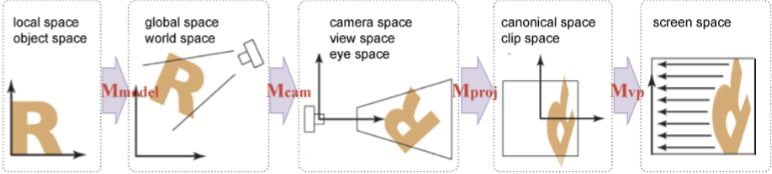
\includegraphics[width=\linewidth]{rendering-steps.png}

\section{Transformations \& Coordinate Systems}
\textbf{Linear Transformation}:
\(
f(\begin{bmatrix}
    x \\ y
\end{bmatrix})
= \begin{bmatrix}
    a_{11} & a_{12} \\
    a_{21} & a_{22}
\end{bmatrix}
\begin{bmatrix}
    x \\ y
\end{bmatrix}
=
\begin{bmatrix}
    a_{11} x + a_{12} y \\
    a_{21} x + a_{22} y
\end{bmatrix}
\)
satisfies: \(
f(\mathbf{u} + \mathbf{v})
= f(\mathbf{u}) + f(\mathbf{v})
\)
and
\(
f(c\mathbf{u}) = cf(\mathbf{u})
\)

In other words, origin is unchanged, straight lines remain straight lines.

\textbf{Affine Transformation}
Straight lines remain lines.

\textbf{2D Rotations}
\(
f(p)
= x \begin{bmatrix}
    \cos \theta \\ \sin \theta
\end{bmatrix}
+ y \begin{bmatrix}
    -\sin \theta \\ \cos \theta
\end{bmatrix}
= \begin{bmatrix}
    \cos \theta & - \sin \theta \\
    \sin \theta & \cos \theta
\end{bmatrix}
\begin{bmatrix}
    x \\ y
\end{bmatrix}
\)

\textbf{3D Rotations}

\textit{Rotate around X}
\(
f(p) = \begin{bmatrix}
    1 & 0           & 0            \\
    0 & \cos \theta & -\sin \theta \\
    0 & \sin \theta & \cos \theta
\end{bmatrix}
\begin{bmatrix}
    x \\ y \\ z
\end{bmatrix}
\)

\textit{Rotate around Y}
\(
f(p) = \begin{bmatrix}
    \cos \theta  & 0 & \sin \theta \\
    0            & 1 & 0           \\
    -\sin \theta & 0 & \cos \theta
\end{bmatrix}
\begin{bmatrix}
    x \\ y \\ z
\end{bmatrix}
\)

\textit{Rotate around Z}
\(
f(p) = \begin{bmatrix}
    \cos \theta & -\sin \theta & 0 \\
    \sin \theta & \cos \theta  & 0 \\
    0           & 0            & 1
\end{bmatrix}
\begin{bmatrix}
    x \\ y \\ z
\end{bmatrix}
\)

For a generic 3D rotation:
\(
R =
\begin{bmatrix}
    ax & bx & cx \\
    ay & by & cy \\
    az & bz & cz
\end{bmatrix}
\)
Where the \(a*\) column is the coordinates of the object's \(x'\) vector,
the \(b*\) column is the \(y'\) vector,
and the \(c*\) column is the \(z'\) vector:
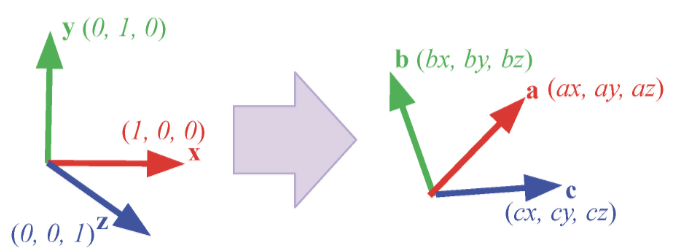
\includegraphics[width=\linewidth]{3d-rotation.png}

\textbf{2D Reflection}
Reflect X:\@
\(
\begin{bmatrix} -1 & 0 \\ 0 & 1 \end{bmatrix}
\)
Reflect Y:\@
\(
\begin{bmatrix} 1 & 0 \\ 0 & -1 \end{bmatrix}
\)

\textbf{3D Scaling}
\(
\begin{bmatrix}
    s_x & 0   & 0   \\
    0   & s_y & 0   \\
    0   & 0   & s_z
\end{bmatrix}
\begin{bmatrix}
    x \\ y \\ z
\end{bmatrix}
=
\begin{bmatrix}
    s_x x \\ s_y y \\ s_z z
\end{bmatrix}
\)

\textbf{2D Shear Matrix}
Horizontal shear (top edge is shifted to the right (positive)):
\(
\begin{bmatrix}
    1 & s_x \\
    0 & 1
\end{bmatrix}
\)
Vertical shear (right edge is shifted up (positive)):
\(
\begin{bmatrix}
    1   & 0 \\
    s_y & 1
\end{bmatrix}
\)

\textbf{3D Shear Matrix}
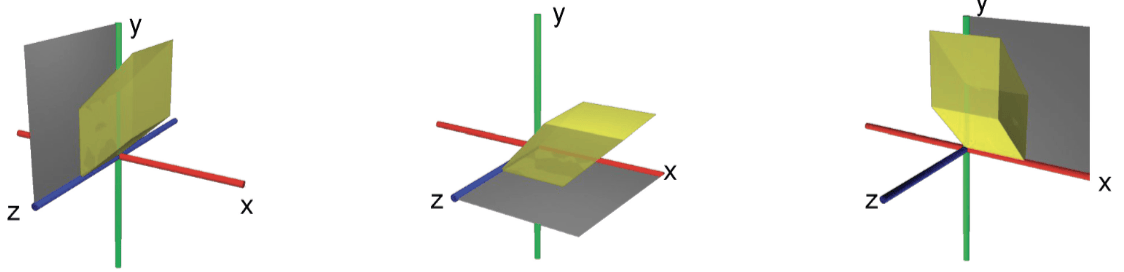
\includegraphics[width=\linewidth]{3d-shear.png}
Shear on YZ Plane:
\(
\begin{bmatrix}
    1   & 0 & 0 \\
    s_y & 1 & 0 \\
    s_z & 0 & 1
\end{bmatrix}
\)

Shear on XZ Plane:
\(
\begin{bmatrix}
    1 & s_x & 0 \\
    0 & 1   & 0 \\
    0 & s_z & 1
\end{bmatrix}
\)

Shear on XY Plane:
\(
\begin{bmatrix}
    1 & 0 & s_x \\
    0 & 1 & s_y \\
    0 & 0 & 1
\end{bmatrix}
\)

\textbf{Homogenous Coordinate}
2D points represented by \((x, y, z)\), 2D location is \((x/z, y/z) \mid z=1\) or other value
3D points represented by \((x, y, z, w)\), 3D location is \((x/w, y/w, z/w) \mid w=1\) or other value
Used for perspective projection, \(z\) becomes depth value.

\textit{Transformation Matrix}
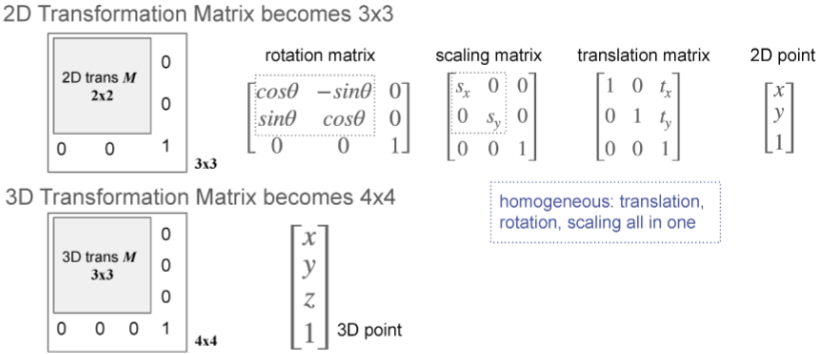
\includegraphics[width=\linewidth]{homogenous-coord-transformation-matrix.png}

\textbf{Composite Transformation}
Since scaling, rotation, etc is about origin, operations are not commutive!

\textit{Examples}
To rotate around an object's centre, 1 translate object centre to origin, 2 rotate, 3 translate back.

To scale an object along a non uniform axis, 1 rotate the object to align with a canonical axis, 2 scale object, 3 rotate object back.

\textbf{Inversions}
For rotation, scaling, and translating,
the inverse of a matrix \(M^{-1}\) can be used.
For rotation specifically, \(M^{-1}_{rotate}=M^T_{rotate}\)
For scaling, inversion is essentially \(1/s\) for your scale factor.
For translating, do \(-x\).

\textbf{Coordinate Systems}
\textit{World/Global Coordinate}
Only one, unique.
Each model in scene goes through \(M_{model}\) to transform from model space to world space.

\section{Camera}

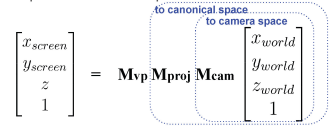
\includegraphics[width=\linewidth]{cam-total.png}

\textbf{Viewing General Steps}
\begin{enumerate}
    \item Model 3D Objects in local space
    \item Put 3D object at world coordinates
    \item View scene in Camera space
    \item Project camera space into cannonical space
    \item Transform cannonical space to screen
\end{enumerate}

\textbf{World Space $\to$ Camera Space: $M_{cam}$}
Given camera position $e$, gaze direction $g$ and `up' direction $t$, construct basis $uwv$ for camera coordinate system.
$w = - \frac{g}{||g||}, u = \frac{t \times w}{||t \times w||}, v = w \times u$

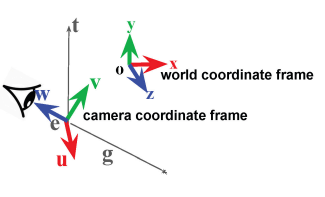
\includegraphics[height=3cm]{camera-basis.png}
% Todo Replace Picture, it's too big

\textit{Camera Space $\to$ World Space:}\\
\(
\begin{bmatrix}
    1 & 0 & 0 & x_e \\
    0 & 1 & 0 & y_e \\
    0 & 0 & 1 & z_e \\
    0 & 0 & 0 & 1   \\
\end{bmatrix}
\)
\(
\begin{bmatrix}
    x_u & x_v & x_w & 0 \\
    y_u & y_v & y_w & 0 \\
    z_u & z_v & z_w & 0 \\
    0   & 0   & 0   & 1 \\
\end{bmatrix}
\)\\

\textbf{World Space $\to$ Camera Space: $M_{cam}=$}\\
\(
\begin{bmatrix}
    x_u & y_u & z_u & 0 \\
    x_v & y_v & z_v & 0 \\
    x_w & y_w & z_w & 0 \\
    0   & 0   & 0   & 1 \\
\end{bmatrix}
\)
\(
\begin{bmatrix}
    1 & 0 & 0 & -x_e \\
    0 & 1 & 0 & -y_e \\
    0 & 0 & 1 & -z_e \\
    0 & 0 & 0 & 1    \\
\end{bmatrix}
\)
\\
Step 1 (left matrix): Translates camera position $e$ to origin $e$. Things originally at $e$ are now at $\vec{0}$.\\
Step 2 (right matrix): Rotates, maps basis vectors: $u \mapsto (1,0,0), v \mapsto (0,1,0), w \mapsto (0,0,1)$

\textbf{3x3 Camera Matrix}
\(
M_{cam}
\begin{bmatrix}
    x_{cam} & y_{cam} & z_{cam}
\end{bmatrix}
\)
Use column vectors

\textbf{Cannonical Space}\\
Cannonical space is the space $(x, y, z)$ s.t. $x,y,z \in [-1, 1]$.

\textbf{Orthographic Projection}\\

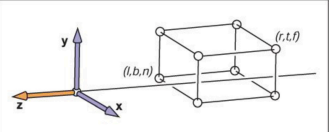
\includegraphics[width=\linewidth]{cam-ortho.png}
Given left plane x, $l$, right plane x, $r$, top plane y, $t$, bottom plane y $b$, near plane $n$, far plane $f$.
\textit{Recall that $f$, $n$ are negative z values. See diagram.}

$M_{orth}$ projects the view box defined above onto the cannonical space.


$M_{orth}$ = \(
\begin{bmatrix}
    \frac{2}{r-l} & 0             & 0             & 0 \\
    0             & \frac{2}{t-b} & 0             & 0 \\
    0             & 0             & \frac{2}{n-f} & 0 \\
    0             & 0             & 0             & 1 \\
\end{bmatrix}
\)
\(
\begin{bmatrix}
    1 & 0 & 0 & -\frac{r+l}{2} \\
    0 & 1 & 0 & -\frac{t+b}{2} \\
    0 & 0 & 1 & -\frac{n+f}{2} \\
    0 & 0 & 0 & 1              \\
\end{bmatrix}
\)\\
=
\(
\begin{bmatrix}
    \frac{2}{r-l} & 0             & 0             & -\frac{r+l}{r-l} \\
    0             & \frac{2}{t-b} & 0             & -\frac{t+b}{t-b} \\
    0             & 0             & \frac{2}{n-f} & -\frac{f+n}{n-f} \\
    0             & 0             & 0             & 1                \\
\end{bmatrix}
\)\\
Right: translate center to origin\\
Left: scales width of all dimensions to be 2, fitting inside [-1, 1].

\textbf{Perspective Projection}\\
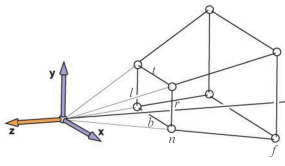
\includegraphics[width=\linewidth]{cam-persp.png}
$l,r,b,t$ now define the near plane $XY$, with $n$ being the $Z$. Far plane is only defined by $f$.
\textbf{OR} use depth of field:
$\theta$ = FOV on y-axis, $ratio = (r-l)/(t-b)$, $n$ is near plane z, $f$ is far plane z.

\textbf{Frustrum to Box:}
Recall Homogenous Coordinates. We want frustrum $\mapsto$ box s.t. $n$ stays near and $f$ stays far.

$P$ =
\(
\begin{bmatrix}
    n & 0 & 0   & 0   \\
    0 & n & 0   & 0   \\
    0 & 0 & n+f & -fn \\
    0 & 0 & 1   & 0   \\
\end{bmatrix}
\)\\
$M_{per}$ = $M_{orth}P =$
\(
\begin{bmatrix}
    \frac{2n}{r-l} & 0              & \frac{l+r}{l-r} & 0               \\
    0              & \frac{2n}{t-b} & \frac{b+t}{b-t} & 0               \\
    0              & 0              & \frac{f+n}{n-f} & \frac{2fn}{n-f} \\
    0              & 0              & 1               & 0               \\
\end{bmatrix}
\)\\

\textbf{Cannonical Space To View Port (VP)}\\

View port is a screen of size $(n_x, n_y)$, no $z$ depth.\\
1. Translate $x,y$ center from $(0,0)$ to $((n_x-1)/2, (n_y-1)/2)$.
2. Scale $x,y$ size from $(2,2)$ to $(n_x, n_y)$.

$M_{vp} = $
\(
\begin{bmatrix}
    \frac{n_x}{2} & 0             & 0 & \frac{n_x-1}{2} \\
    0             & \frac{n_y}{2} & 0 & \frac{n_y-1}{2} \\
    0             & 0             & 1 & 0               \\
    0             & 0             & 0 & 1               \\
\end{bmatrix}
\)\\



\section{Rasterization}

\textit{Definition:} finding all pixels on the screen that are occupied by a geometric primitive.

\textbf{Bi-linear Interpolation}
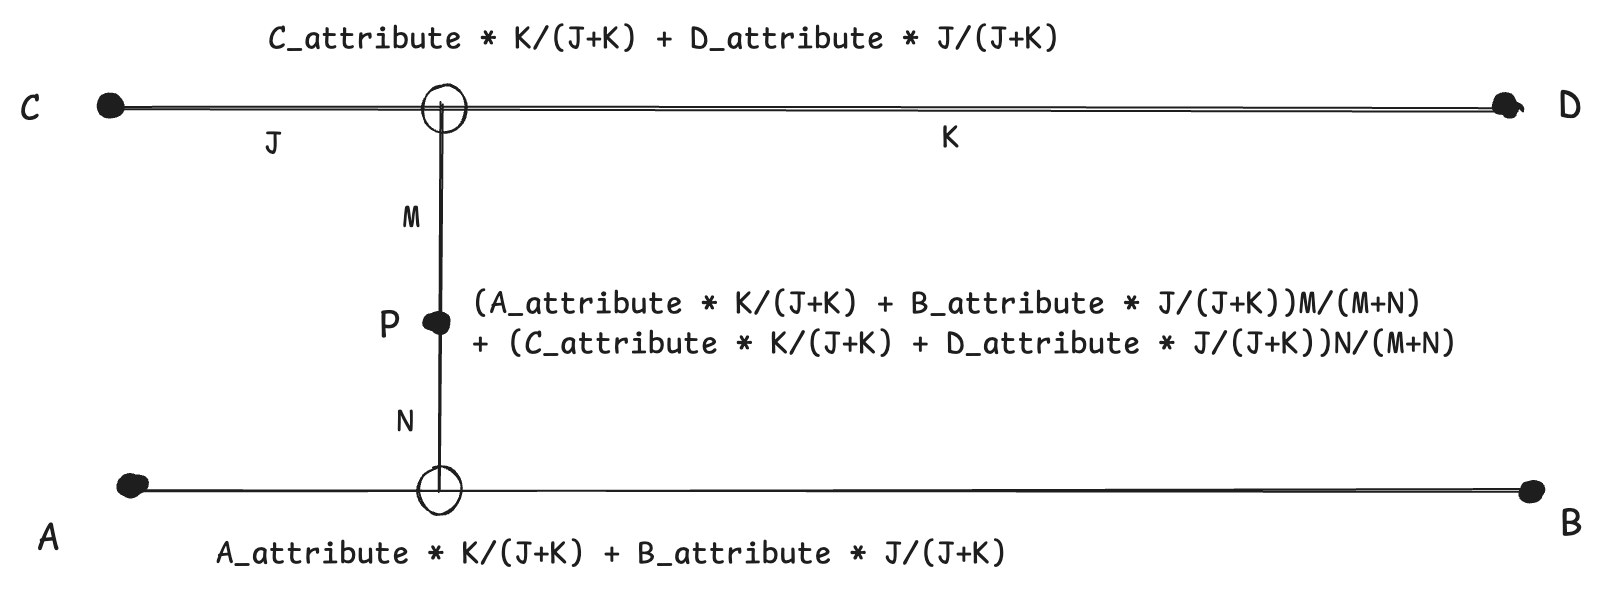
\includegraphics[width=\linewidth]{bilinear-interpolation.png}

\textbf{Line Rasterization}
Given pixels $P_0 = (x_0, y_0), P_1 = (x_1, y_1)$, fill the pixels on the screen between them.

$f(x, y): y = mx + c$\\given $m=(y_1 - y_0)/(x_1 - x_0), c=(x_1y_0 - x_0y_1)/(x_1 - x_0)$\\begin{align*}
Implicitly, $f(x,y): Ax + By - C = 0$

\textbf{Naive Implementation:} Use the function $y=mx+c$ and iterate $x$ from $x_0$ to $x_1$. No vertical lines!\\
\textbf{Digital Difference Analyser DDA:} Similar, but move in the axis that is shallower.

% 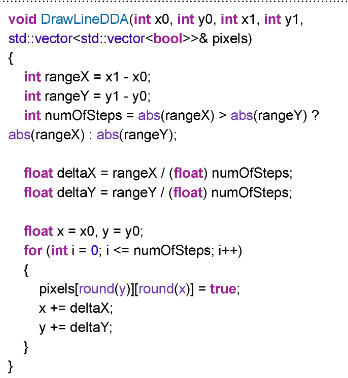
\includegraphics[width=\linewidth]{rasterize-dda.png} 
\begin{lstlisting}
drawDDA(p0, p1):
    ranges = p1-p0
    numSteps = (ranges.x > ranges.y) 
        ? ranges.x
        : ranges.y

    delta = ranges / numSteps
    p = p0

    for i in 0..numSteps:
        fill pixel (round(p.x), round(p.y))
        p += delta
\end{lstlisting}

\textbf{Midpoint Algorithm:} Assume $x_0 < x_1$. Otherwise, swap $P_0, P_1$.
Seperate cases based on $m$ either $\in \{(-\infty, -1], (-1, 0],(0, 1], (1, \infty)\}$.
The case will affect which pixels are the candidate pixels.

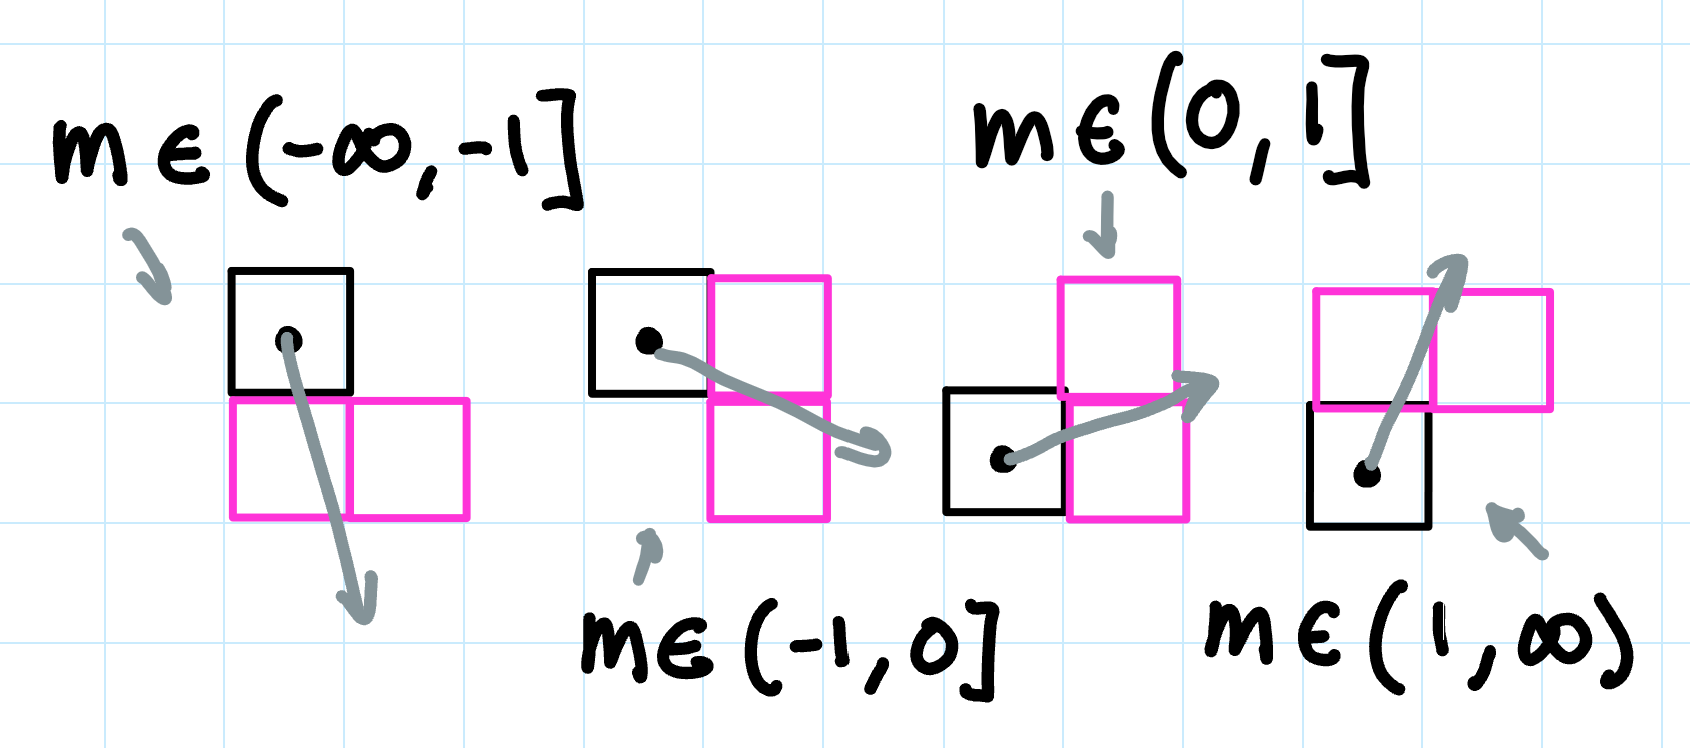
\includegraphics[width=\linewidth]{rasterize-candidates.png}\\
For following cases, assume $m \in [0, 1)$.

Assume $(x, y)$ is drawn. Compute the midpoint of the next candidates, in this case $(x+1, y+0.5)$

To check if point is above line, calculate if $f(x+1, y+0.5) > 0$. Otherwise, count it as below. Select the candidate and draw it.

\begin{lstlisting} 
drawMidpointTraditional(x0, y0, x1, y1):
    y = y0
    for x=x0; x<=x1; x++:
        fill pixel (x,y)

        float f = (y0-y1)*(x+1) 
                + (x1-x0)*(y+0.5) 
                + x0*y1 
                - x1*y0

        if (f < 0): 
            y++;
\end{lstlisting}


\textbf{Midpoint Incremental Algorithm:} We don't need to evaluate $f$ at every case, since $m$ is constant.
evaluate $f$ at the first midpoint. We know that our next candidates are either on the same level or above the last candidate.
If we increase diagonal, then $f(x+1, y+1) = f(x,y) + (y_0 - y_1) + (x_1 - x_0)$. If we increase horizontal, then $f(x+1, y) = f(x, y) + (y_1 - y_0)$

% 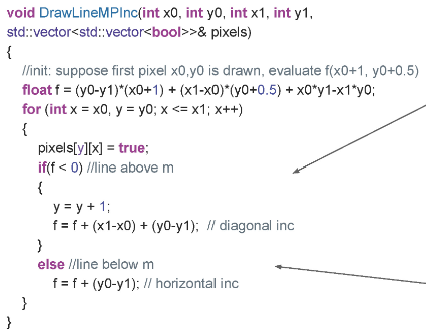
\includegraphics[width=\linewidth]{rasterize-iteration.png}\\
\begin{lstlisting}
drawMidpointIter(x0, y0, x1, x0):
    p = p0
    f = (y0 - y1)*(x0 + 1) 
        + (x1 - x0)*(y0+0.5) 
        + x0*y1
        - x1*y0

    y = y0
    for x = x0; x <= x1; x++:
        fill pixels[x][y]
        if (f < 0): //line above M
            f += (x1-x0) + (y0-y1) 
            y++;
        else: //line below M
            f += y0-y1
\end{lstlisting}

\textbf{Bresenham Algorithm:}

% 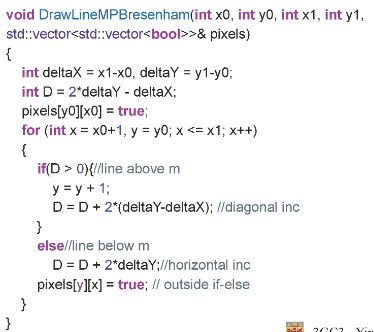
\includegraphics[width=\linewidth]{rasterize-bresen.png}\\
\begin{lstlisting} 
drawBresenham(x0, y0, x1, y1):
    deltaX = x1-x0
    deltaY = y1-y0
    D = 2*deltaY - deltaX

    fill pixel (x0,y0)
    y = y0

    for x=x0+1; x<=x1; x++:

        //Diagonal Increment
        if D > 0:
            y++
            D += 2*(deltaY-deltaX)

        //H Increment
        else:
            D += 2*deltaY
        
        fill pixel (x,y)
\end{lstlisting}

\textbf{Triangle Rasterization}

First, we find the bounding box (rectangle) of the triangle using the min and max positions of all 3 vertexes.
Then, we iterate over every pixel ($n^2$), checking if the barycentric coordinate of the pixel lies inside the triangle.

We can tell if it's outside if all coordinates are $\geq 0$. If one is not, then it is outside, and we skip drawing.

The rest of the following code interpolates the colour of the pixels (p0 is red, p1 is green and p2 is blue).


\begin{lstlisting}[language=C++]
void DrawTriangle(int x0, int y0, 
        int x1, int y1, 
        int x2, int y2, 
        std::vector<std::vector<std::string>> &pixels) {

// Bounding box
int minx = std::min({x0, x1, x2});
int maxx = std::max({x0, x1, x2});
int miny = std::min({y0, y1, y2});
int maxy = std::max({y0, y1, y2});

// Precompute terms for barycentric coordinates
float F01 = (y0-y1)*x2 + (x1-x0)*y2 + x0*y1 - x1*y0;
float F12 = (y1-y2)*x0 + (x2-x1)*y0 + x1*y2 - x2*y1;
float F20 = (y2-y0)*x1 + (x0-x2)*y1 + x2*y0 - x0*y2;

// Vertex colors: p0 - Red, p1 - Green, p2 - Blue
int R0 = 255, G0 = 0, B0 = 0;  // p0 - Red
int R1 = 0, G1 = 255, B1 = 0;  // p1 - Green
int R2 = 0, G2 = 0, B2 = 255;  // p2 - Blue

// Loop over bounding box pixels
for (int x = minx; x <= maxx; ++x) {
    for (int y = miny; y <= maxy; ++y) {

        // Calculate barycentric coordinates
        float f01 = (y0-y1)*x + (x1-x0)*y + x0*y1 - x1*y0;
        float f12 = (y1-y2)*x + (x2-x1)*y + x1*y2 - x2*y1;
        float f20 = (y2-y0)*x + (x0-x2)*y + x2*y0 - x0*y2;

        float b0 = f12 / F12, b1 = f20 / F20, b2 = f01 / F01;

        // Check if inside the triangle
        if (b0 >= 0 && b1 >= 0 && b2 >= 0) {
            // Interpolate color
            int R = b0*R0 + b1*R1 + b2*R2;
            int G = b0*G0 + b1*G1 + b2*G2;
            int B = b0*B0 + b1*B1 + b2*B2;

            // Set pixel color
            pixels[y][x] = std::to_string(R) + ',' +
                            std::to_string(G) + ',' +
                            std::to_string(B);
        }
    }
}
}
\end{lstlisting}


\textbf{Non-overlapping Triangles sharing edges:} We want to ensure no-double drawing.
Assume $T_1, T_2$ share one edge. Let $a$ be the vertex of $T_1$ not along this edge. Let $b$ be the coresponding vertex in $T_2$.
Choose offscreen point $q$.

$T_1$ should be responsible of drawing the edge if $q$ falls on the same side of the edge as $a$. Likewise for $T_2$ and $b$.

\textbf{Proper Perspective Attribute Attribution}: How we set up the above code leads to incorect attribute interpolation when taking perspective into account.
This is because we are interpolating on the 2d projection of the triangle and not considering the distace of the 3d space.

We can interpolate using the following code, which scales based on a scaling metric.

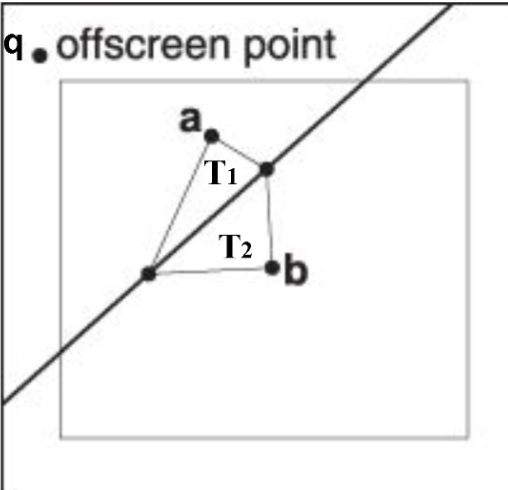
\includegraphics[width=.5\linewidth]{rasterize-triangle-edge.png}

\begin{lstlisting}
float Rs = 60*(R0/w0) + b1*(R1/w1) + b2*(R2/w2);
float Gs = b0*(G0/w0) + b1*(G1/w1) + b2*(G2/w2);
float Bs = 60*(B0/w0) + b1*(B1/w1) + b2*(B2/w2);
float Is = b0*(1/w0) + b1*(1/w1) + b2*(1/w2);

float R = Rs / Is;
float G = Gs / Is;
float B = Bs / Is;
\end{lstlisting}


\textbf{Anti-Aliasing}\\
\textbf{Supersample: }Screen Goal is 256x256. We instead render x4, meaing we actually render a 1024x1024 image.
Then, on scale down, we can average* the 16 virtual pixels into 1 screen pixel.
Can use box filter or a gaussian filter.\\
\textbf{Subsample / Multisample: }
Screen goal is 256x256. We still rasterize for a higher resolution, but fragment (triangle) colour computation is only calculated once.
Then, we sample $n$ times from the pixel area, averaging the samples to get the true pixel colour.


\section{Pipeline}
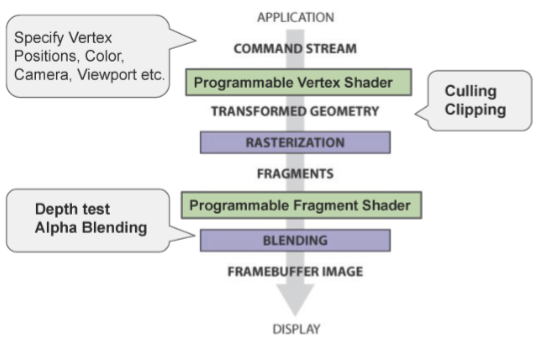
\includegraphics[width=\linewidth]{basic-graphics-pipeline.png}

\subsection{Application}
\textit{Main Program}
Runs on CPU
Defines geometry vertex positions, normals, texture coords, colours, etc.
Sets up camera position, orientation, projection volume
Sets screen size

Copies data to GPU

\subsection{Vertex Shader}
\textit{Per-vertex Computation}
No transformation: Simply assigns input to output (pass-through shader)
Transforming vertex: Apply \(M_{proj} M_{cam} M_{model}\) to input
Shading: determines vertex color (Gouraud)

GPU performs parallel processing on each vertex

\subsection{Culling}
\subsubsection{Backface Culling}
Removes primitives facing away from camera
Look at face normal / right hand rule,
face normal points in same direction as face.

\subsubsection{View Frustrum Culling}
Removes geometries outside view volume.
6 planes: near, far, left, right, top, bottom.
Plane function is
\(
f(p) = n \cdot (p - a)
= n \cdot p + n \cdot a
= n \cdot p + D
= 0
\)
\textbf{Test if outside view volume}
Take bounding box of object, e.g. a sphere with centre c, radius r.
Check \(f(c)\), \(c\)'s signed distance to plane, see if it intersects or is within frustrum.

\subsubsection{Clipping}
View volume cuts primitive to avoid drawing out of bounds

\textbf{Clipping a Line}
\textit{Plane Function}:
\(f(p) = n \cdot p + D = 0\), \(p\) is any point on the plane,
\(n\) is the normal, \(D\) is a known const.

\textit{Line Function}:
\(p(t) = \mathbf{a} + t (\mathbf{b} - \mathbf{a})\)

\textit{Intersection Point}
Plug \(p\) into plane function \(f(p) = n \cdot (\mathbf{a} + t(\mathbf{b} - \mathbf{a})) + D = 0\)
Solve for \(t = \frac{n \cdot \textbf{a} + D}{n \cdot (\textbf{a} - \textbf{b})}\)

\textbf{Clipping a Triangle}

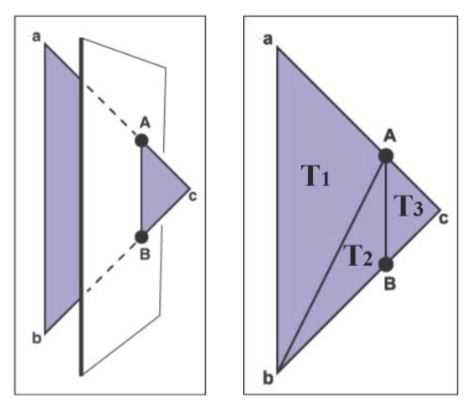
\includegraphics[width=.5\linewidth]{triangle-clipping.png}

\textit{Plane Function}:
Same as above

\textit{Intersection}:
Assume \(a, b\) is on one side, \(c\) is on the other side
Compute intersection points \(\mathbf{A}, \mathbf{B}\) using line clipping method.

\textit{Split Triangle}
\(\mathbf{T}_1=\triangle abA, \mathbf{T}_2=\triangle bBA, \mathbf{T}_3\)

\textit{Throw Away}
If \(f(c) \geq 0\), keep \(T_3\); if \(f(c) < 0\), keep \(\mathbf{T}_1, \mathbf{T}_2\)

\textit{Special Case}
Handle zero-area triangles

\end{multicols*}

\end{document}
